% Options for packages loaded elsewhere
\PassOptionsToPackage{unicode}{hyperref}
\PassOptionsToPackage{hyphens}{url}
%
\documentclass[
]{article}
\usepackage{amsmath,amssymb}
\usepackage{iftex}
\ifPDFTeX
  \usepackage[T1]{fontenc}
  \usepackage[utf8]{inputenc}
  \usepackage{textcomp} % provide euro and other symbols
\else % if luatex or xetex
  \usepackage{unicode-math} % this also loads fontspec
  \defaultfontfeatures{Scale=MatchLowercase}
  \defaultfontfeatures[\rmfamily]{Ligatures=TeX,Scale=1}
\fi
\usepackage{lmodern}
\ifPDFTeX\else
  % xetex/luatex font selection
\fi
% Use upquote if available, for straight quotes in verbatim environments
\IfFileExists{upquote.sty}{\usepackage{upquote}}{}
\IfFileExists{microtype.sty}{% use microtype if available
  \usepackage[]{microtype}
  \UseMicrotypeSet[protrusion]{basicmath} % disable protrusion for tt fonts
}{}
\makeatletter
\@ifundefined{KOMAClassName}{% if non-KOMA class
  \IfFileExists{parskip.sty}{%
    \usepackage{parskip}
  }{% else
    \setlength{\parindent}{0pt}
    \setlength{\parskip}{6pt plus 2pt minus 1pt}}
}{% if KOMA class
  \KOMAoptions{parskip=half}}
\makeatother
\usepackage{xcolor}
\usepackage[margin=1in]{geometry}
\usepackage{graphicx}
\makeatletter
\def\maxwidth{\ifdim\Gin@nat@width>\linewidth\linewidth\else\Gin@nat@width\fi}
\def\maxheight{\ifdim\Gin@nat@height>\textheight\textheight\else\Gin@nat@height\fi}
\makeatother
% Scale images if necessary, so that they will not overflow the page
% margins by default, and it is still possible to overwrite the defaults
% using explicit options in \includegraphics[width, height, ...]{}
\setkeys{Gin}{width=\maxwidth,height=\maxheight,keepaspectratio}
% Set default figure placement to htbp
\makeatletter
\def\fps@figure{htbp}
\makeatother
\setlength{\emergencystretch}{3em} % prevent overfull lines
\providecommand{\tightlist}{%
  \setlength{\itemsep}{0pt}\setlength{\parskip}{0pt}}
\setcounter{secnumdepth}{-\maxdimen} % remove section numbering
\ifLuaTeX
  \usepackage{selnolig}  % disable illegal ligatures
\fi
\IfFileExists{bookmark.sty}{\usepackage{bookmark}}{\usepackage{hyperref}}
\IfFileExists{xurl.sty}{\usepackage{xurl}}{} % add URL line breaks if available
\urlstyle{same}
\hypersetup{
  pdftitle={exploration\_remove\_one\_dataset},
  pdfauthor={Louis Schroll},
  hidelinks,
  pdfcreator={LaTeX via pandoc}}

\title{exploration\_remove\_one\_dataset}
\author{Louis Schroll}
\date{2024-02-12}

\begin{document}
\maketitle

\hypertarget{pelmed-samm-pnm-migralion}{%
\paragraph{PELMED + SAMM + PNM +
MIGRALION}\label{pelmed-samm-pnm-migralion}}

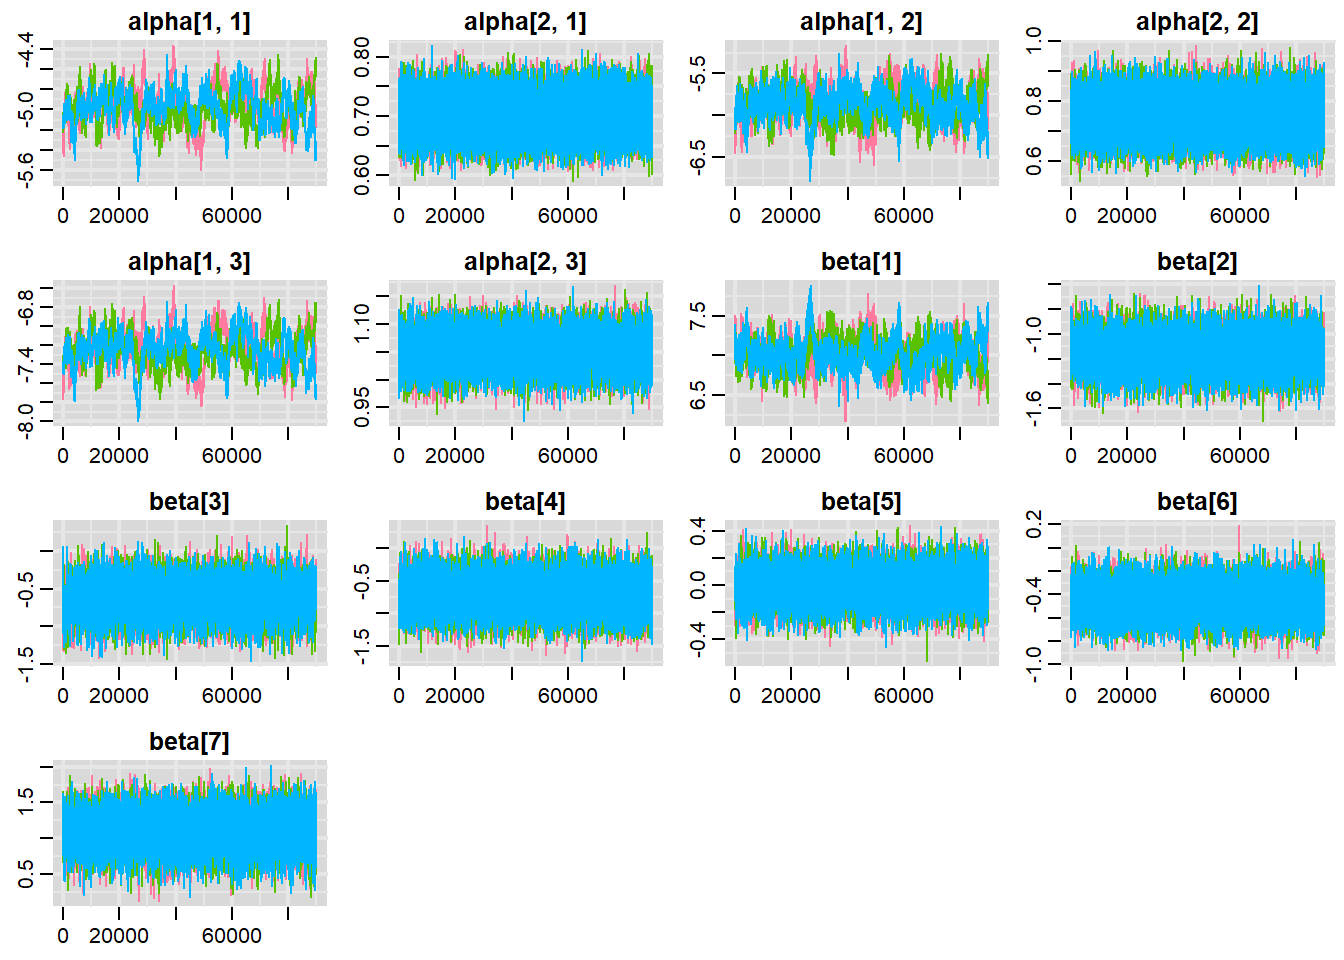
\includegraphics{exploration_remove_one_dataset_files/figure-latex/unnamed-chunk-3-1.pdf}
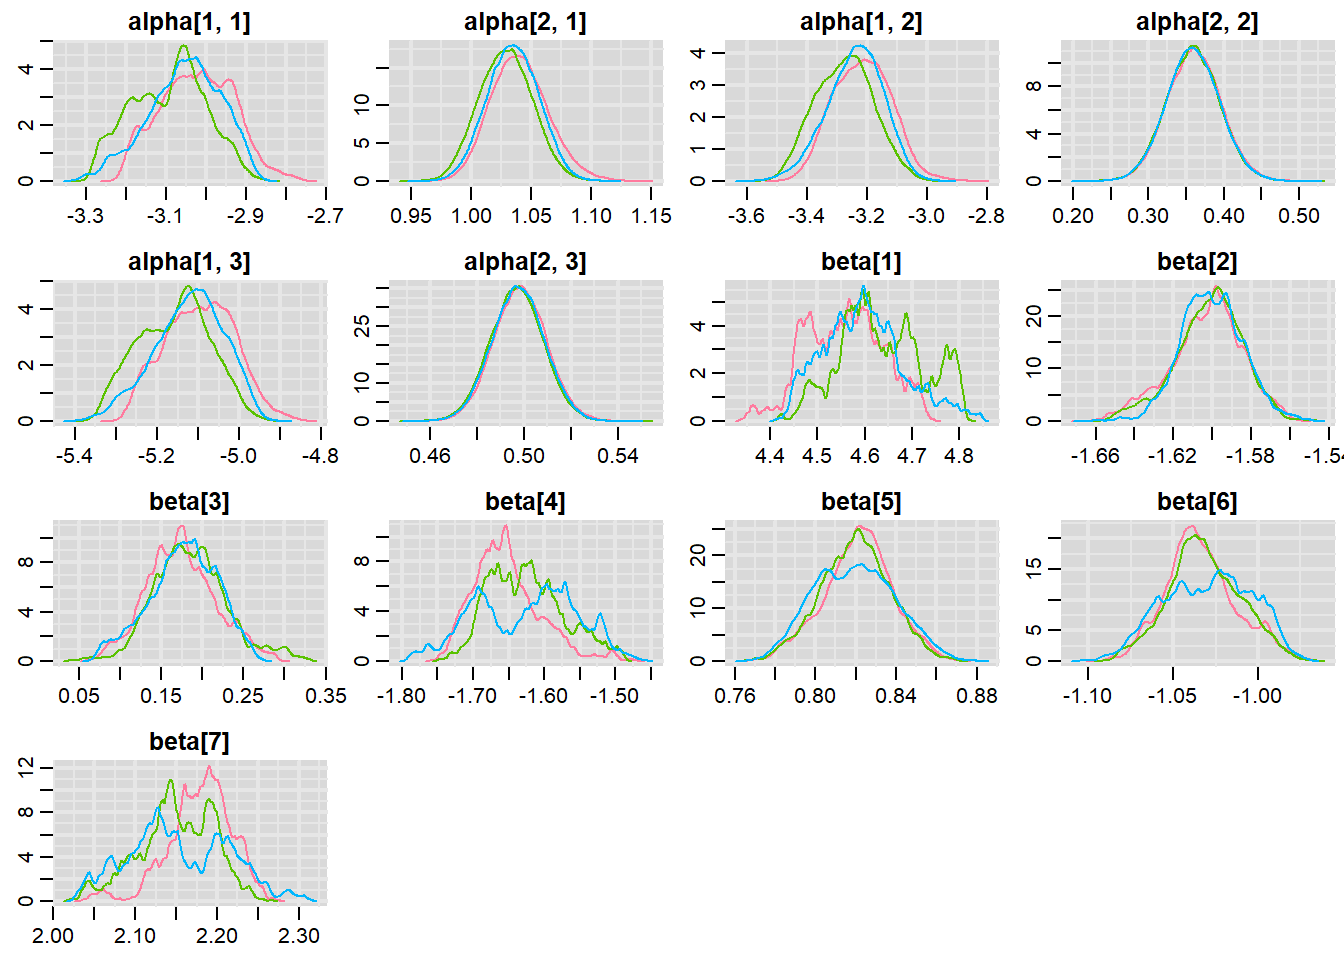
\includegraphics{exploration_remove_one_dataset_files/figure-latex/unnamed-chunk-3-2.pdf}

\hypertarget{pelmed-samm-migralion}{%
\paragraph{PELMED + SAMM + MIGRALION}\label{pelmed-samm-migralion}}

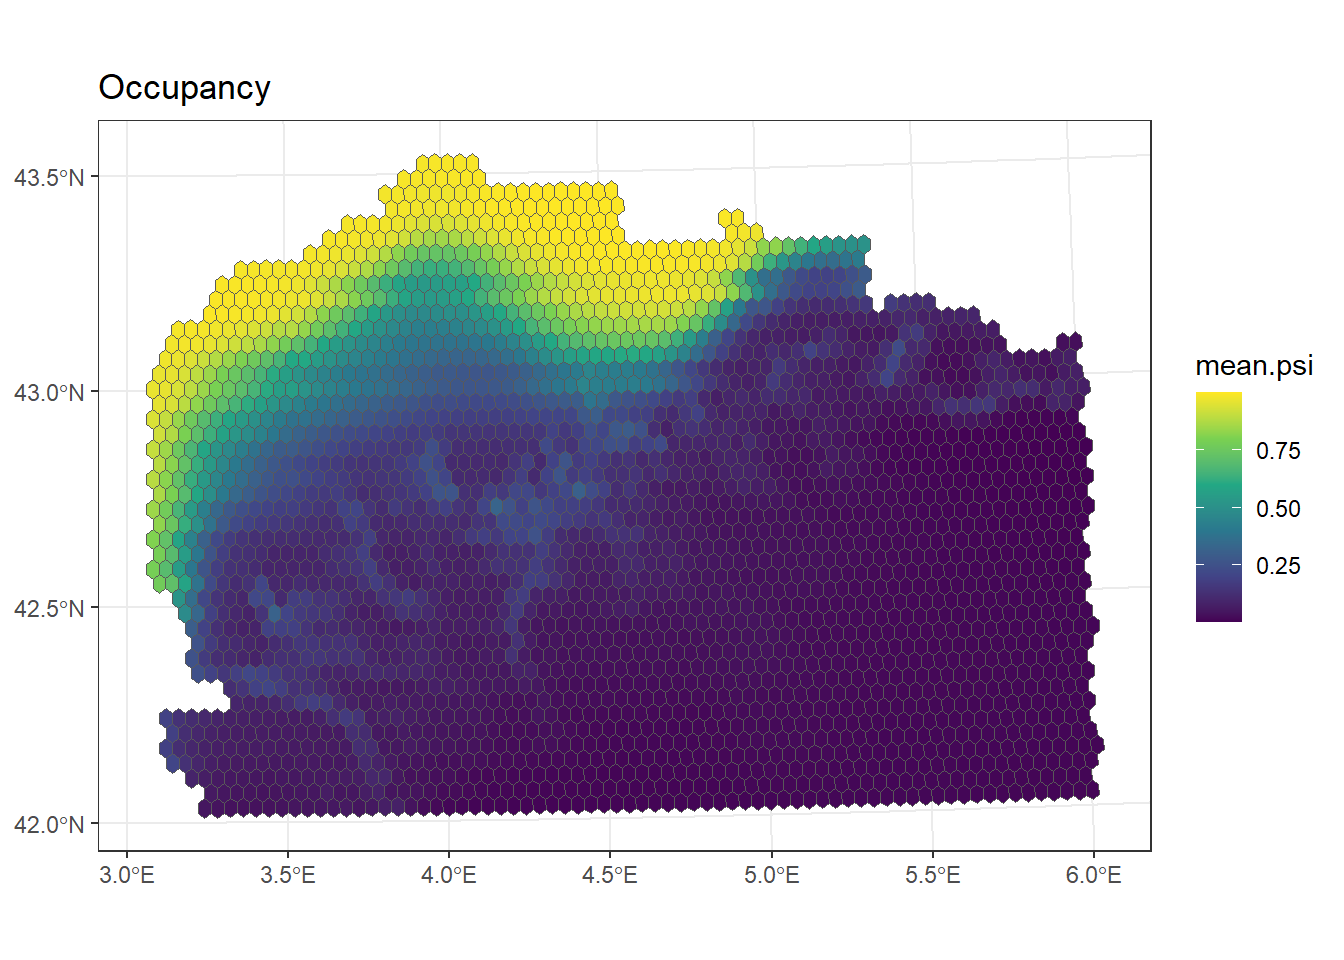
\includegraphics{exploration_remove_one_dataset_files/figure-latex/unnamed-chunk-5-1.pdf}
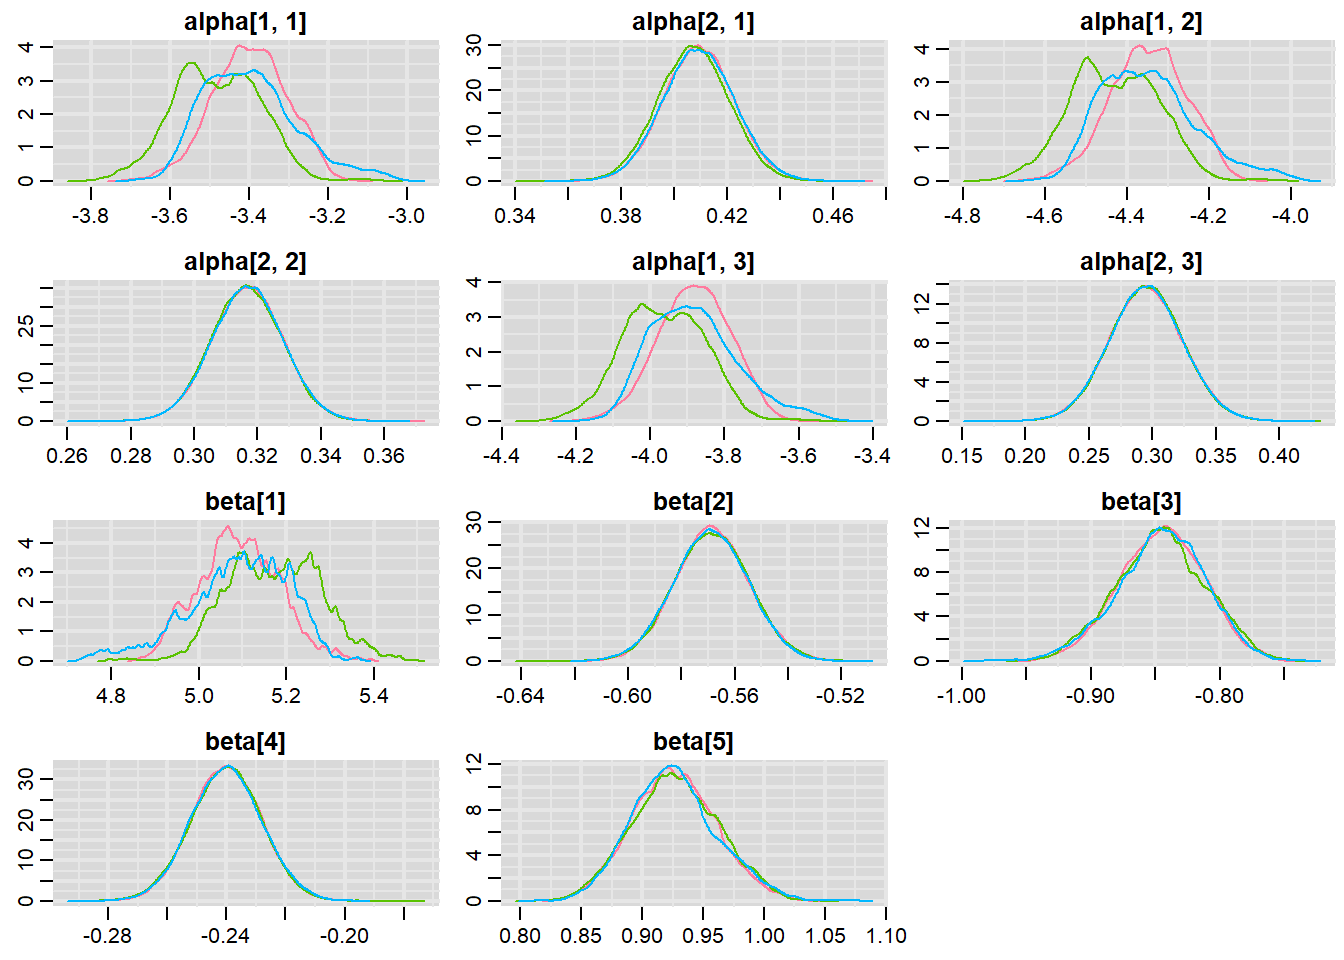
\includegraphics{exploration_remove_one_dataset_files/figure-latex/unnamed-chunk-5-2.pdf}

\hypertarget{pelmed-pnm-migralion}{%
\paragraph{PELMED + PNM + MIGRALION}\label{pelmed-pnm-migralion}}

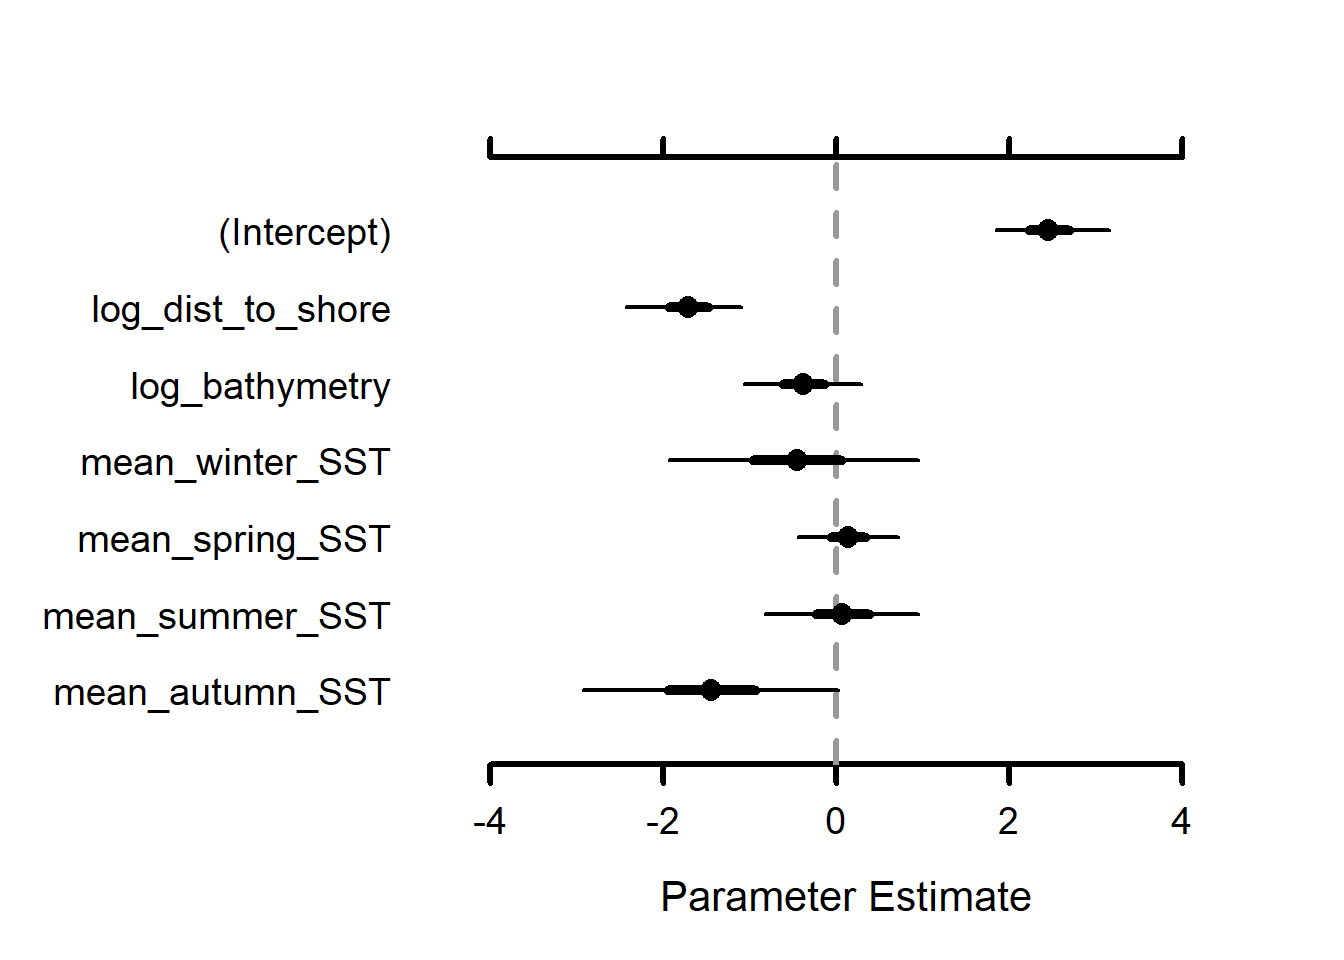
\includegraphics{exploration_remove_one_dataset_files/figure-latex/unnamed-chunk-7-1.pdf}
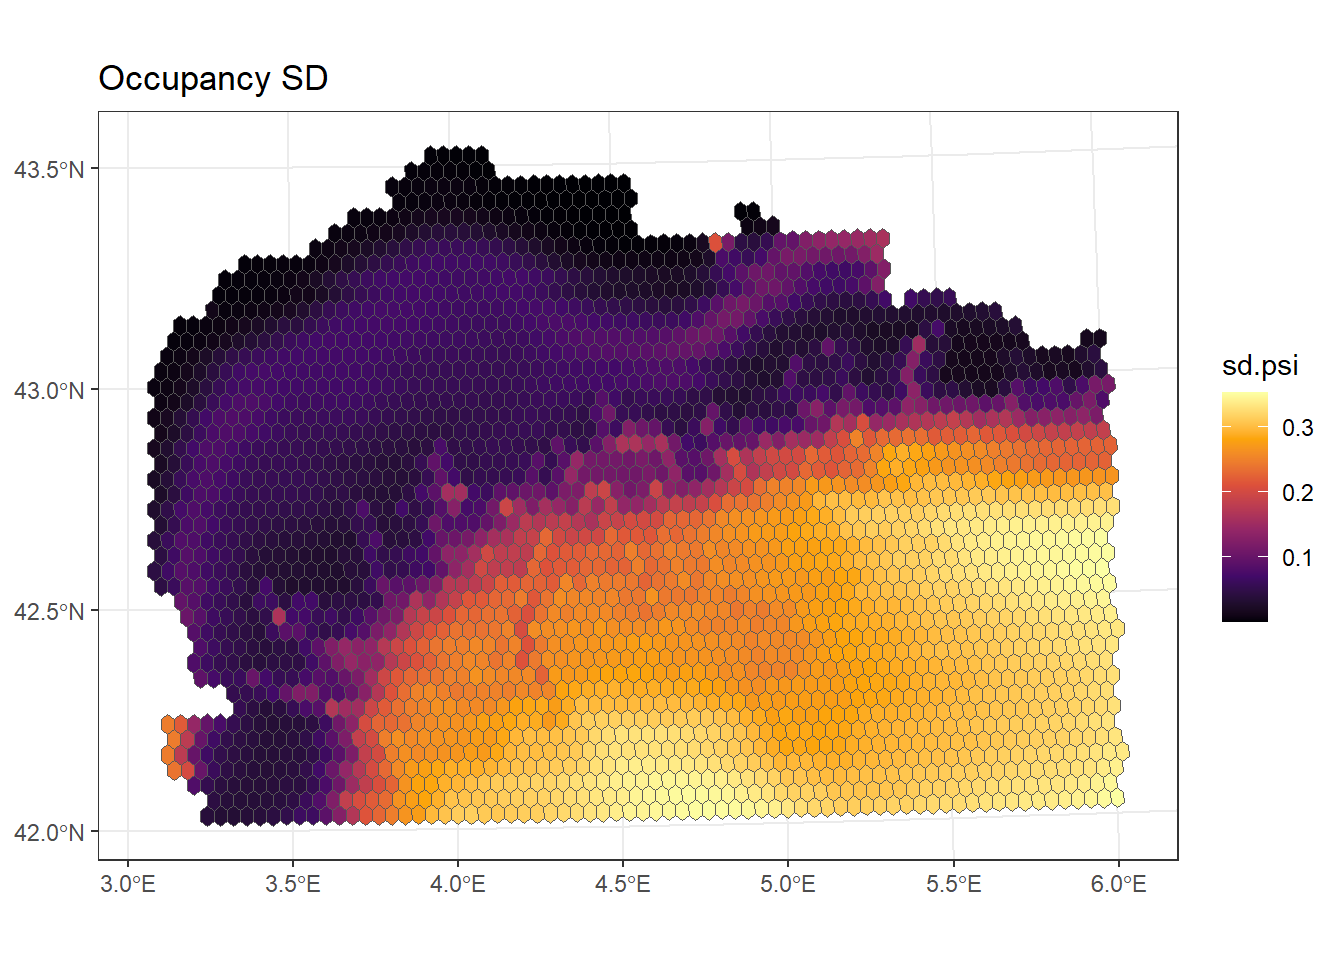
\includegraphics{exploration_remove_one_dataset_files/figure-latex/unnamed-chunk-7-2.pdf}

\hypertarget{samm-pnm-migralion}{%
\paragraph{SAMM + PNM + MIGRALION}\label{samm-pnm-migralion}}

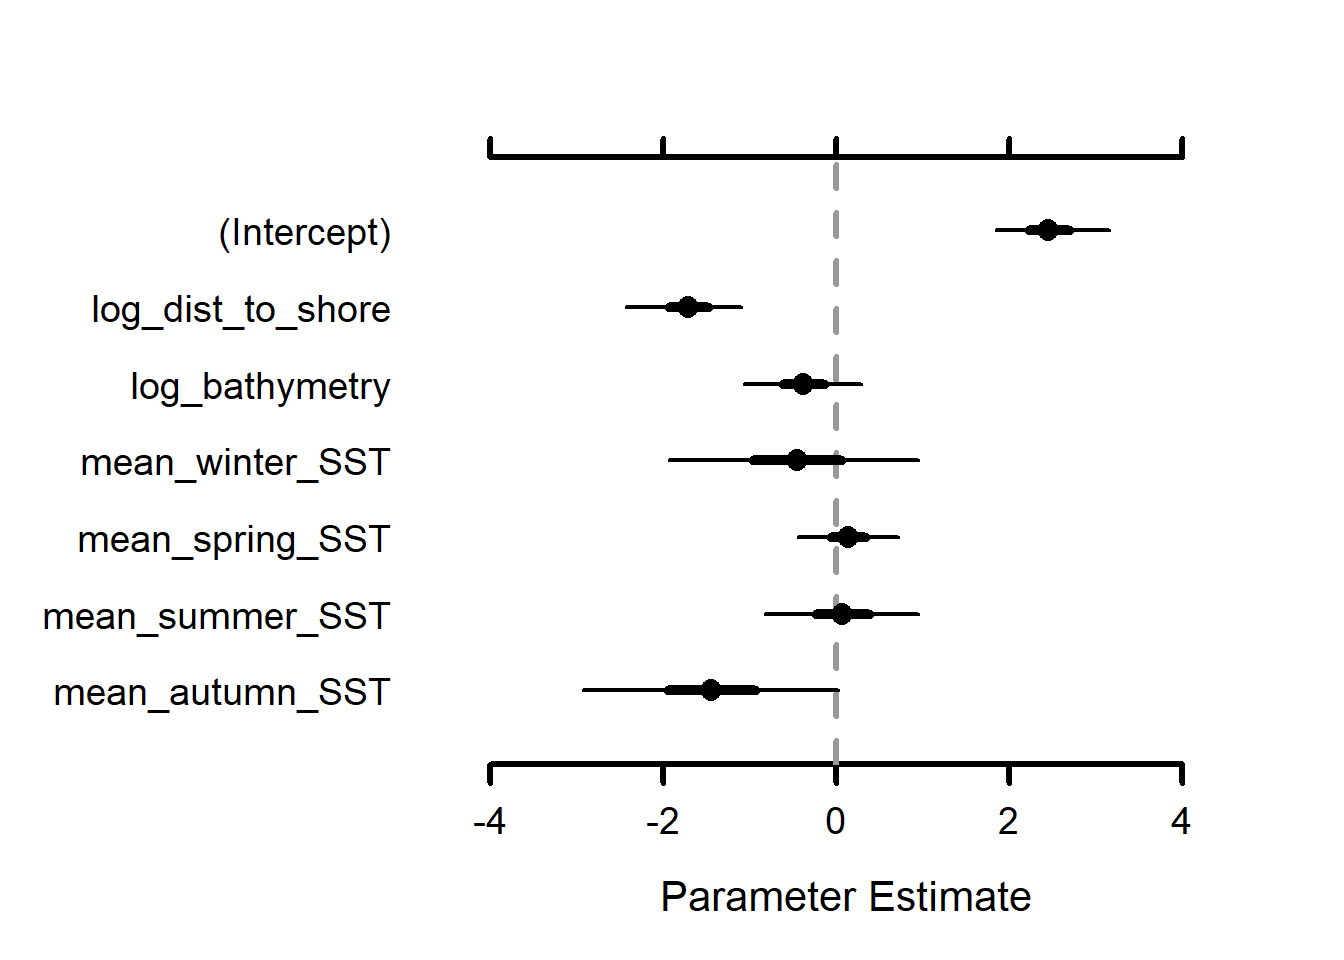
\includegraphics{exploration_remove_one_dataset_files/figure-latex/unnamed-chunk-9-1.pdf}
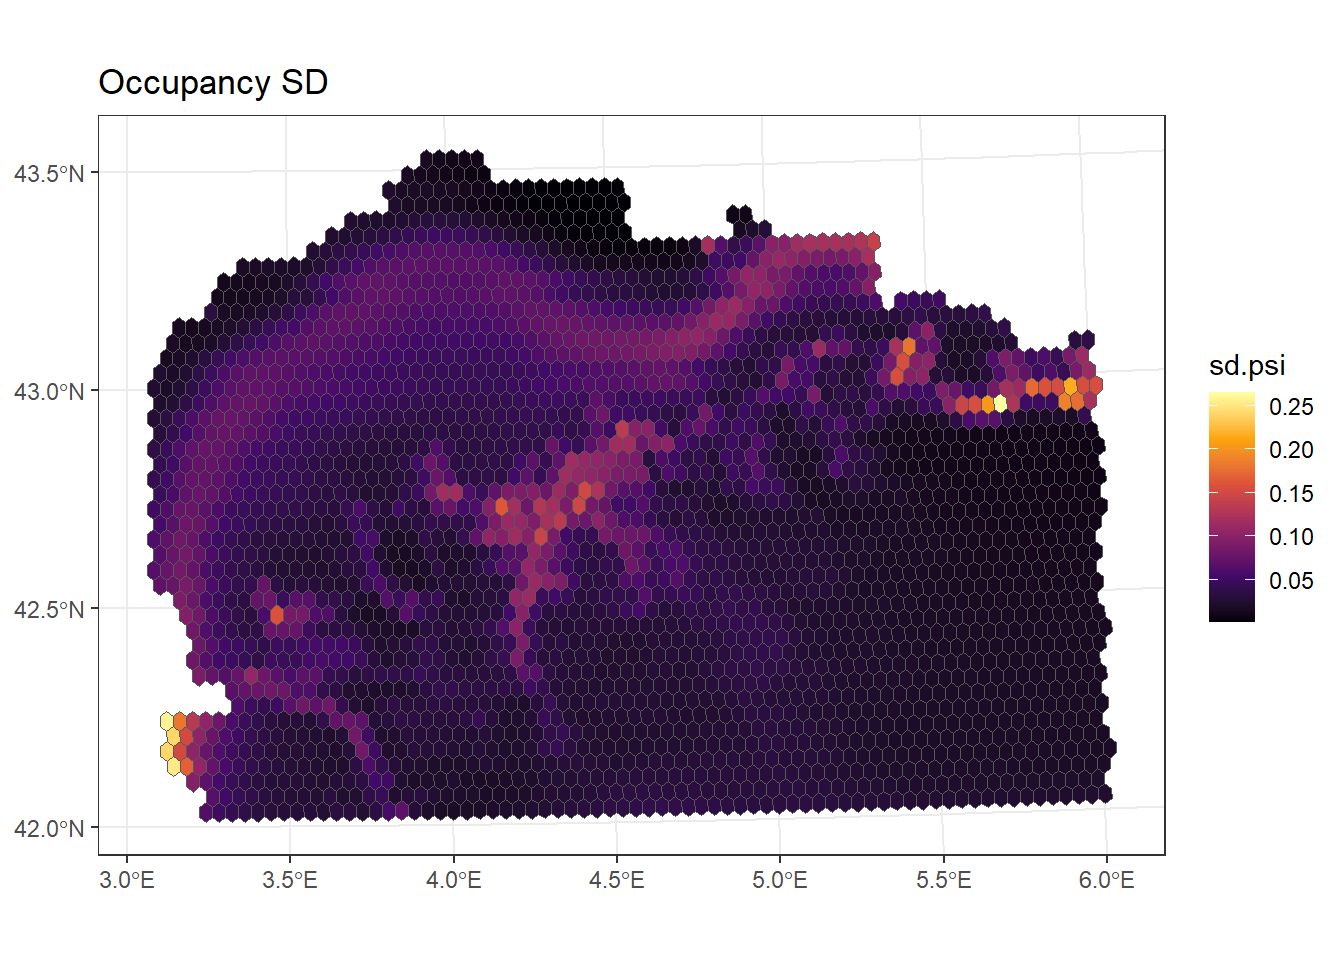
\includegraphics{exploration_remove_one_dataset_files/figure-latex/unnamed-chunk-9-2.pdf}

\hypertarget{pelmed-samm-pnm}{%
\paragraph{PELMED + SAMM + PNM}\label{pelmed-samm-pnm}}

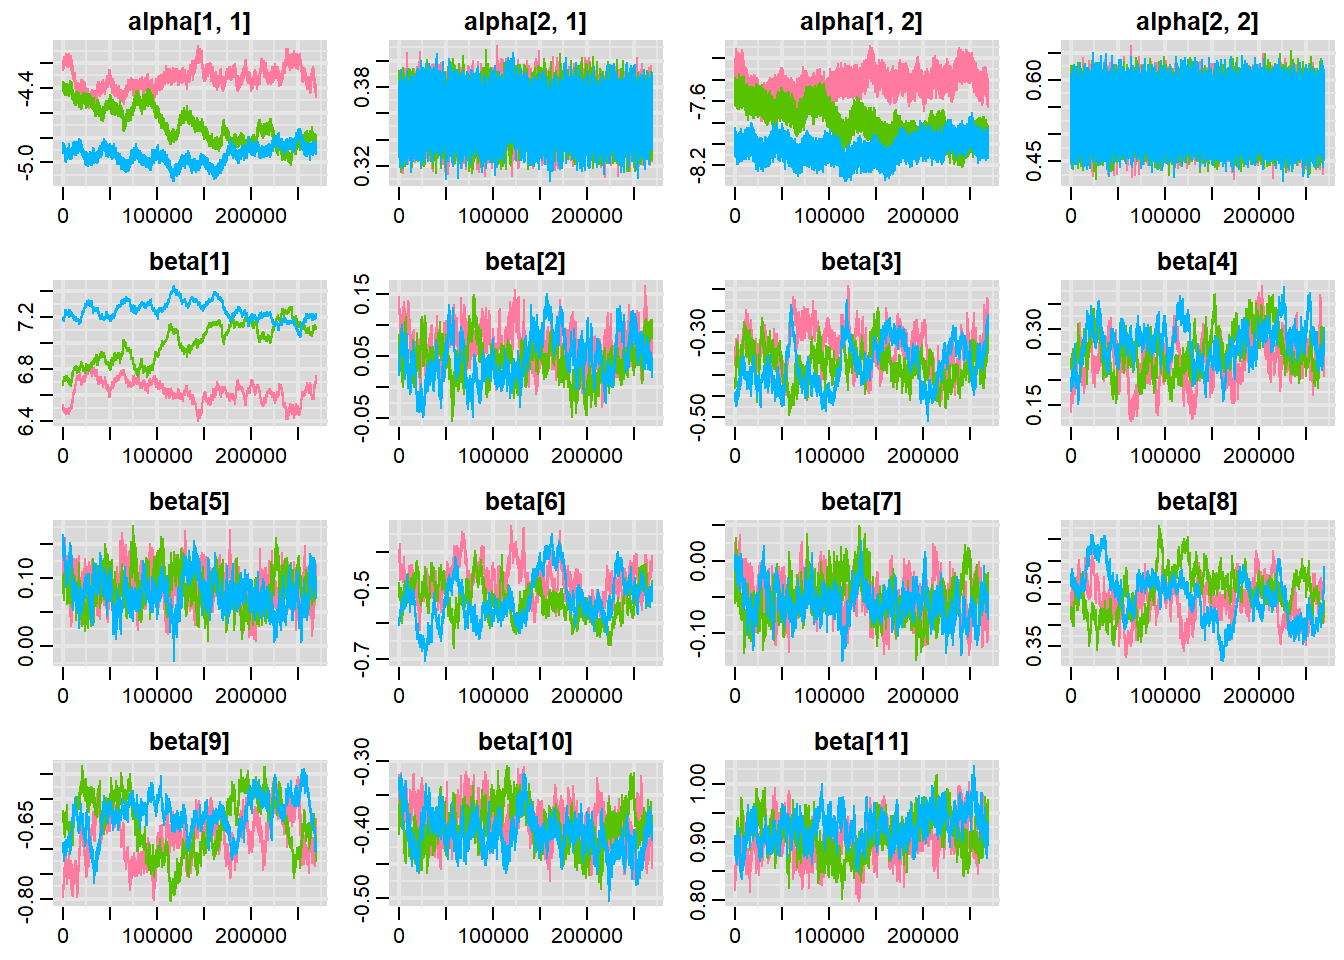
\includegraphics{exploration_remove_one_dataset_files/figure-latex/unnamed-chunk-11-1.pdf}
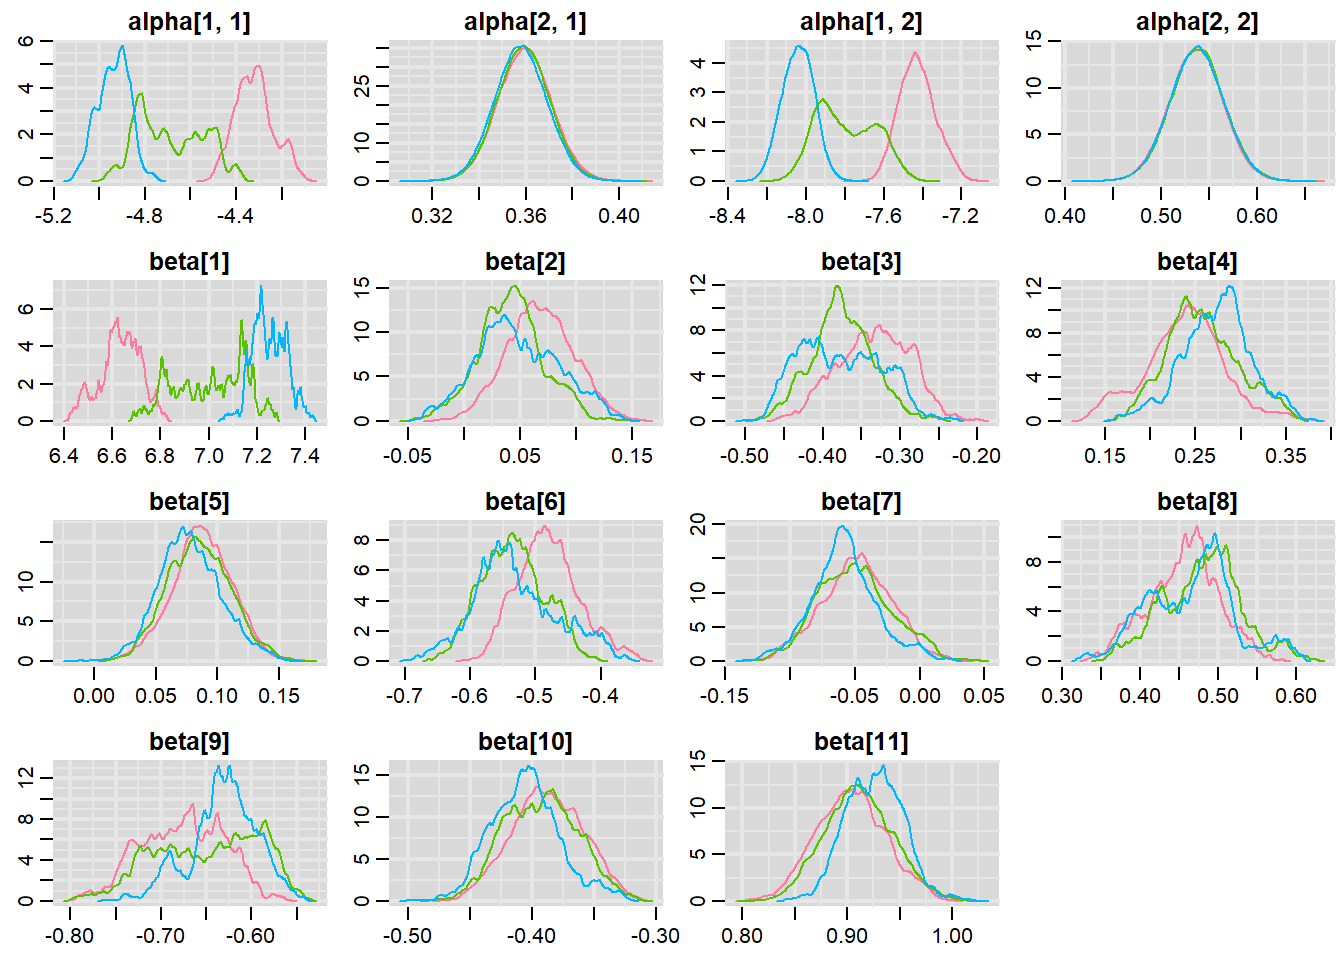
\includegraphics{exploration_remove_one_dataset_files/figure-latex/unnamed-chunk-11-2.pdf}

\hypertarget{pelmed-samm}{%
\paragraph{PELMED + SAMM}\label{pelmed-samm}}

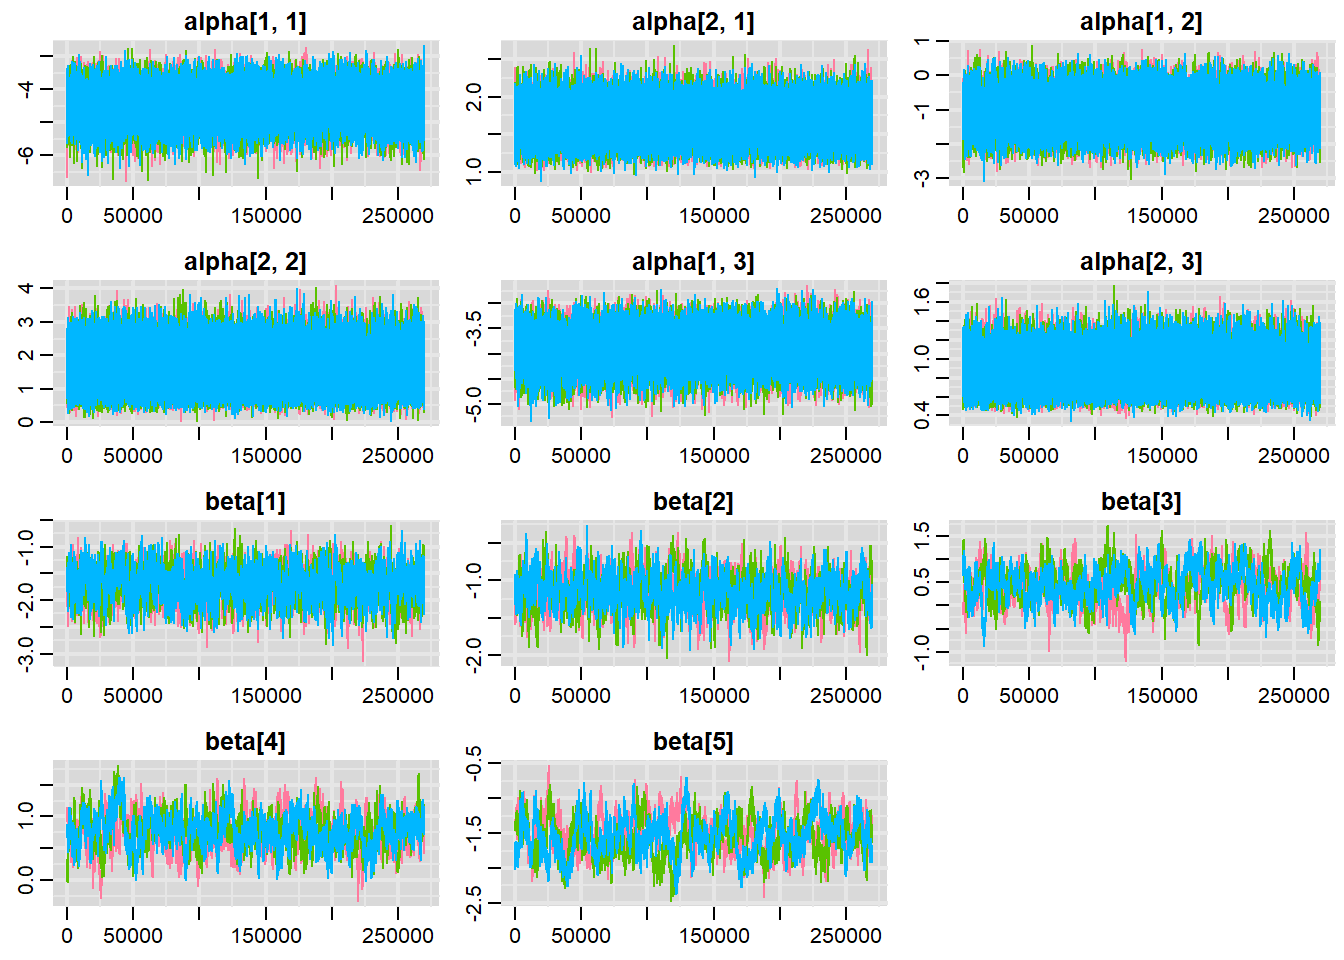
\includegraphics{exploration_remove_one_dataset_files/figure-latex/unnamed-chunk-13-1.pdf}
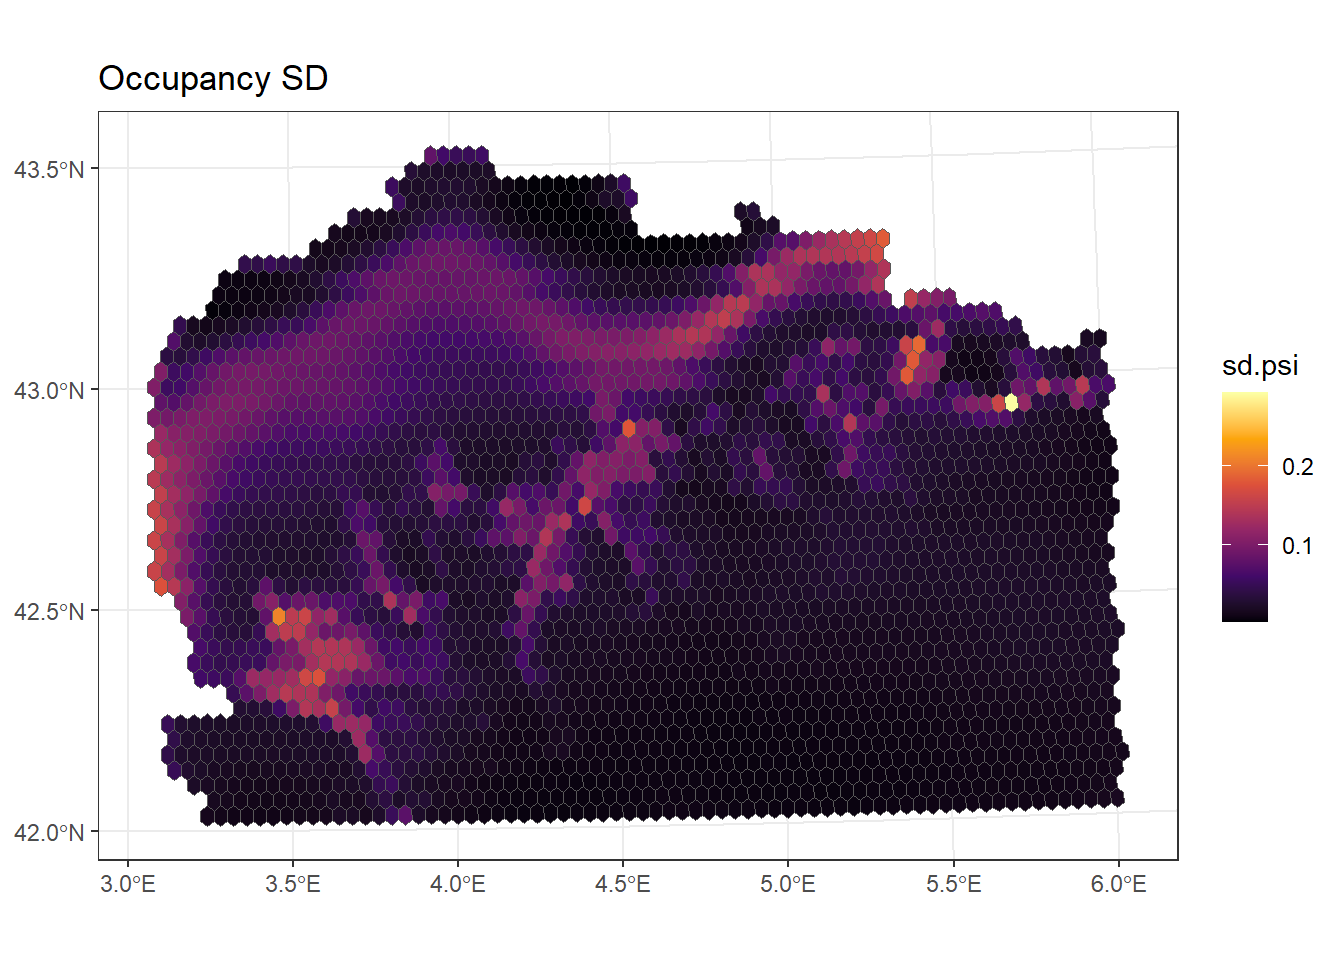
\includegraphics{exploration_remove_one_dataset_files/figure-latex/unnamed-chunk-13-2.pdf}

\hypertarget{pelmed-pnm}{%
\paragraph{PELMED + PNM}\label{pelmed-pnm}}

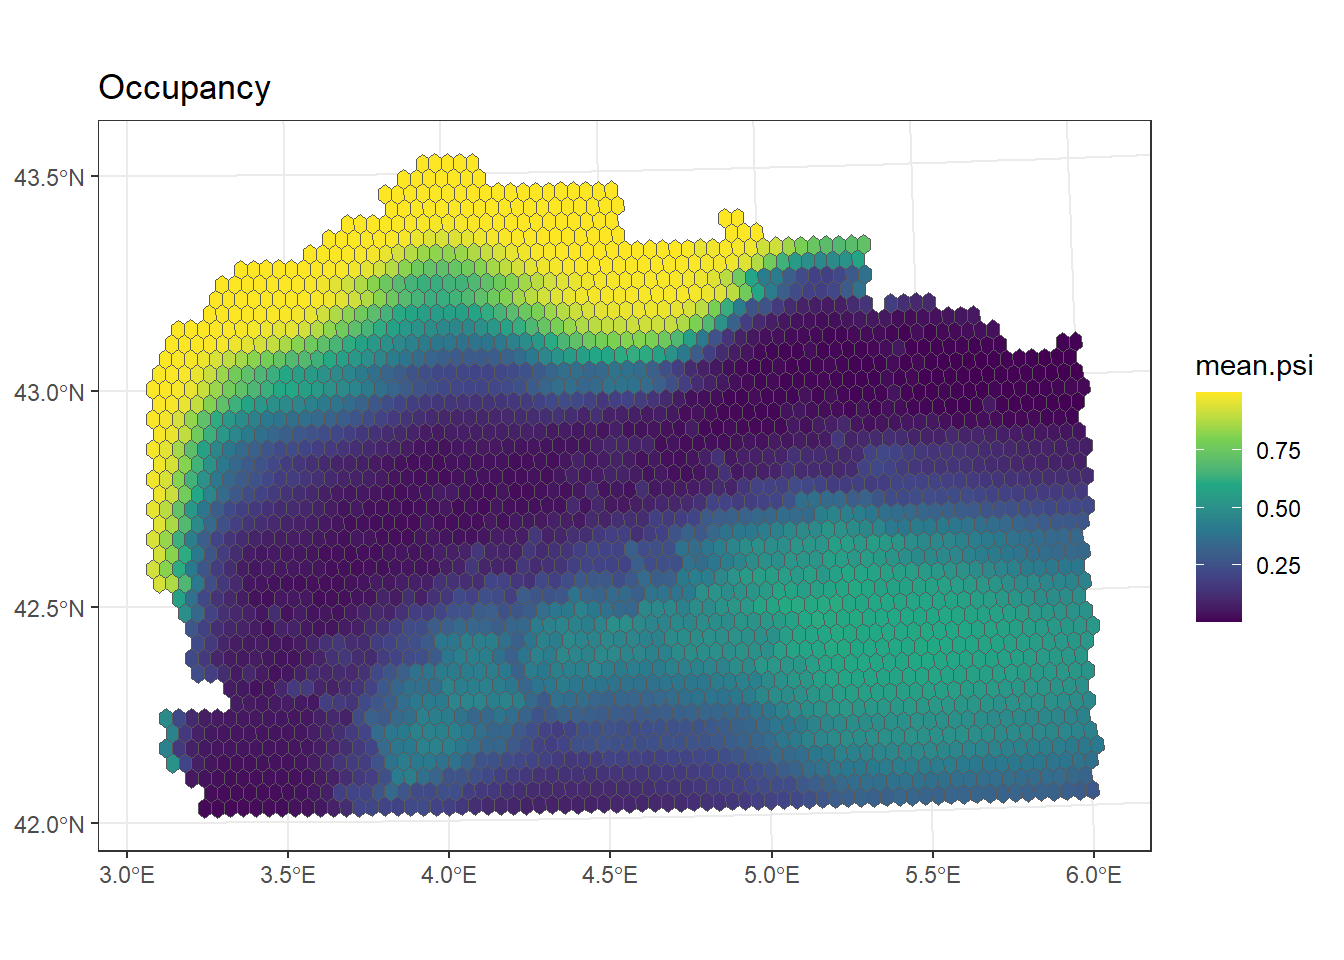
\includegraphics{exploration_remove_one_dataset_files/figure-latex/unnamed-chunk-15-1.pdf}
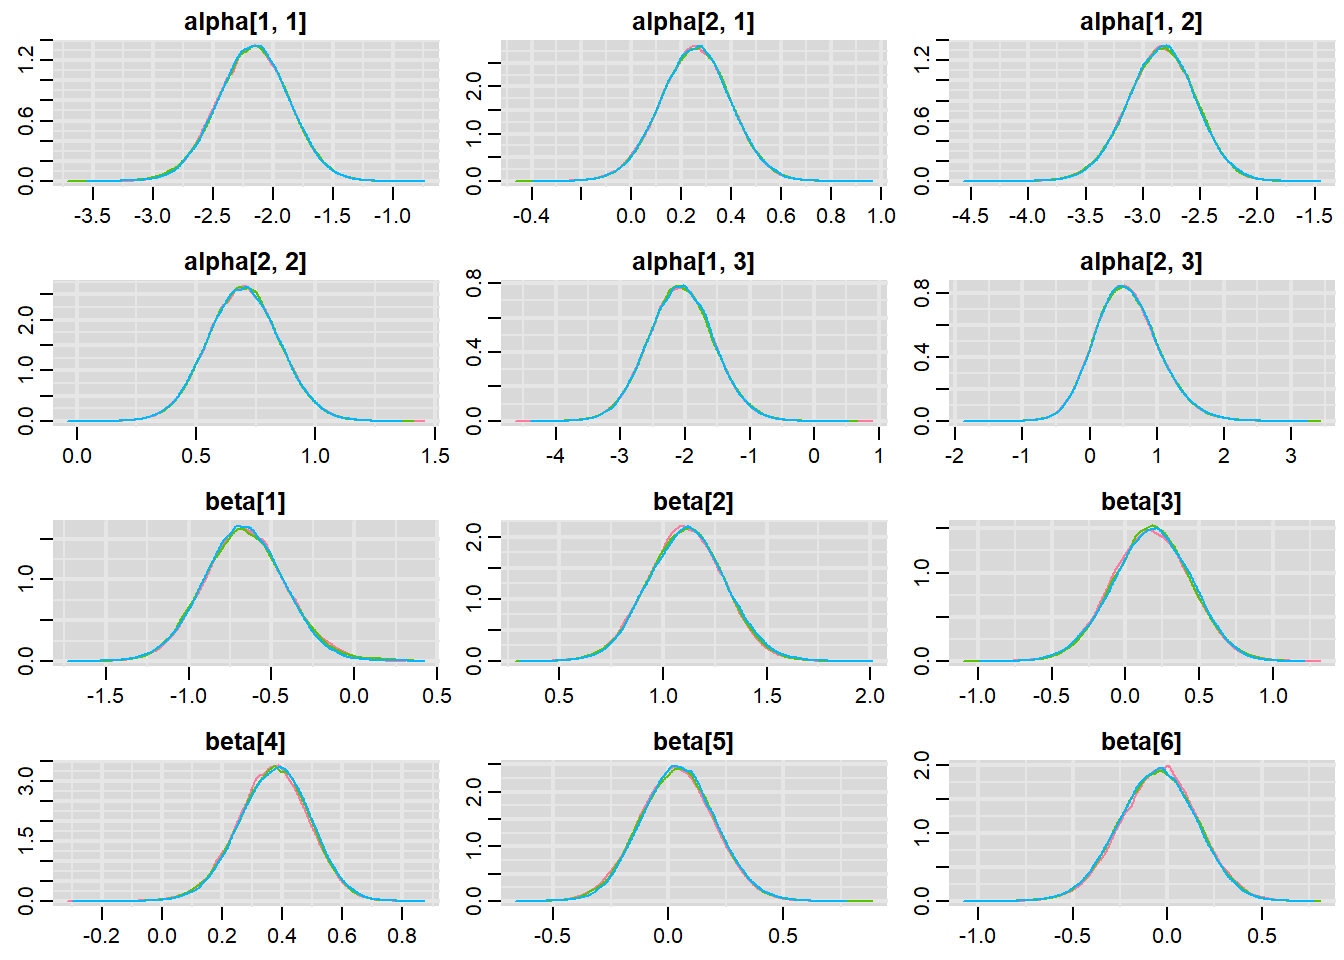
\includegraphics{exploration_remove_one_dataset_files/figure-latex/unnamed-chunk-15-2.pdf}

\hypertarget{pelmed-migralion}{%
\subsubsection{PELMED + MIGRALION}\label{pelmed-migralion}}

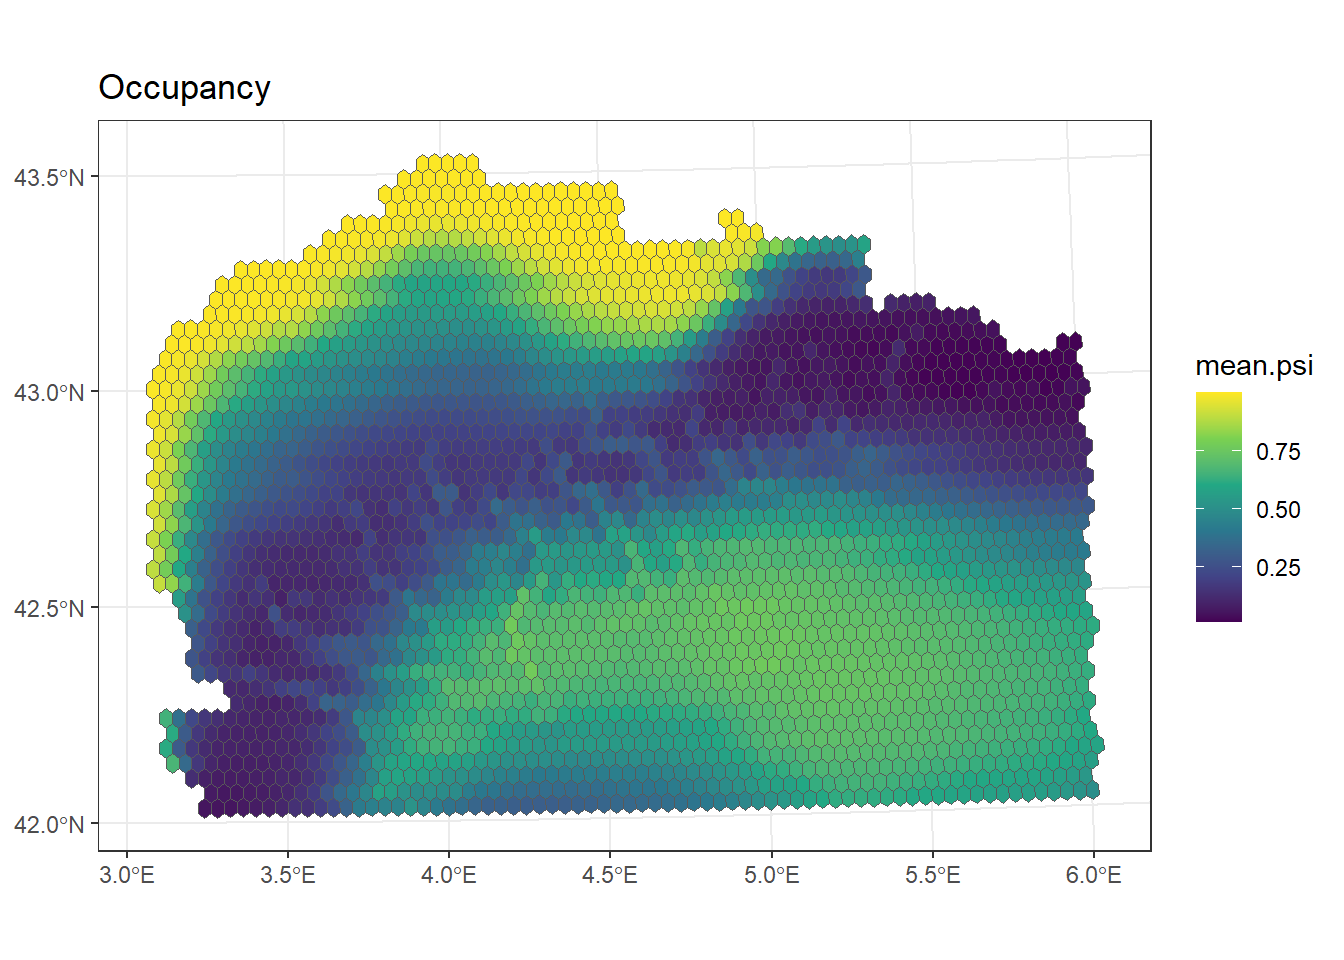
\includegraphics{exploration_remove_one_dataset_files/figure-latex/unnamed-chunk-17-1.pdf}
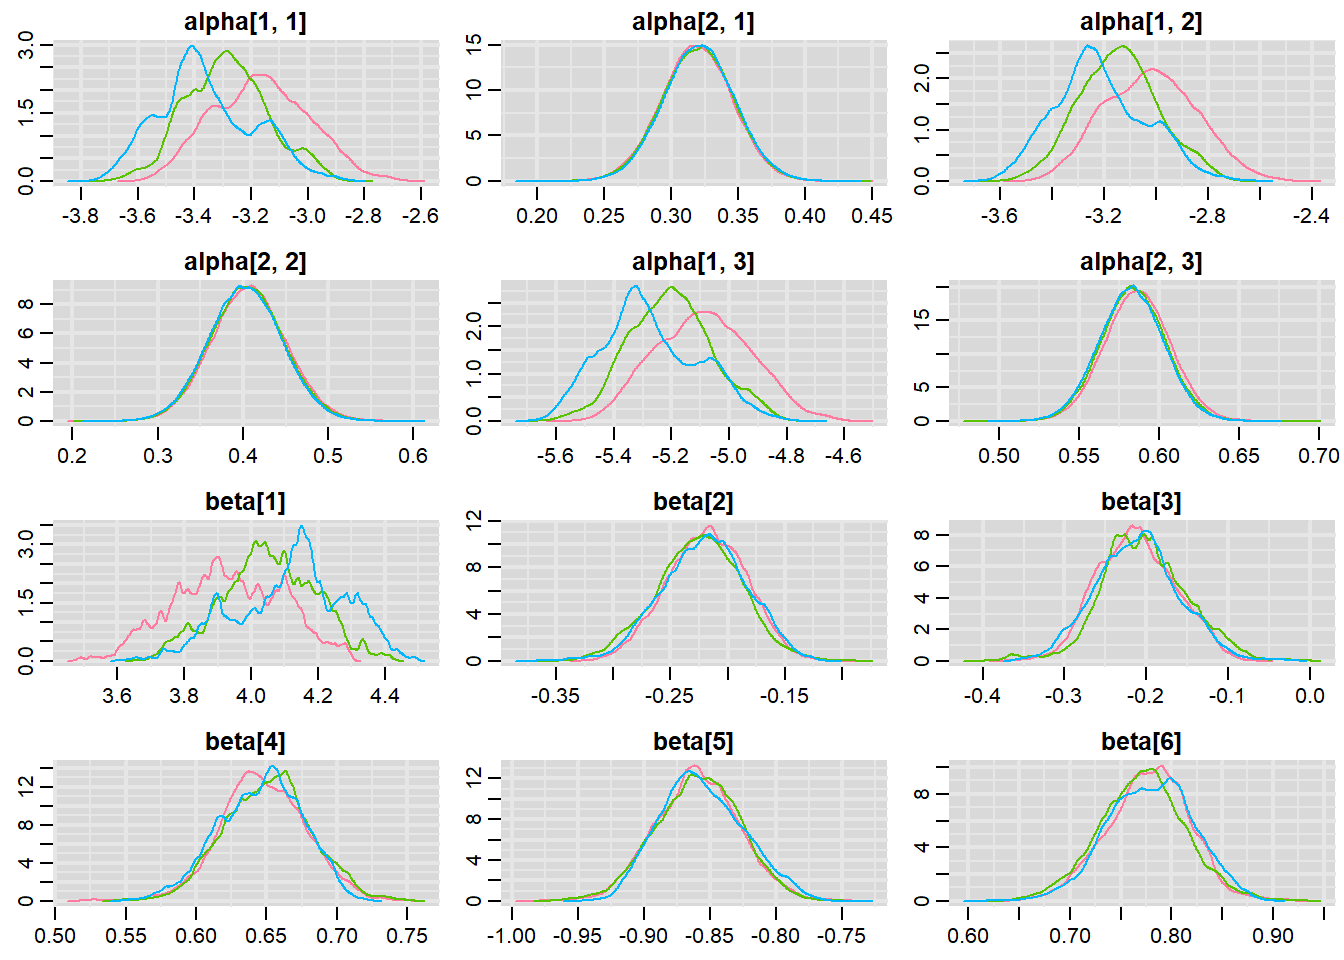
\includegraphics{exploration_remove_one_dataset_files/figure-latex/unnamed-chunk-17-2.pdf}

\end{document}
